% !TEX program = xelatex
% !TEX encoding = UTF-8
% =====================================================================
%  WPA3-SAE 기반 PQC 하이브리드 키 교환 프로토콜 명세 (Draft)
%  Repository: protocol/  (80211-pqc)
%  License: 문서 CC-BY-4.0 / 예제 코드 MIT
%
%  권장 컴파일:  xelatex wpa3-pqc-sae-hybrid.tex   (2회)
%              또는  pdflatex wpa3-pqc-sae-hybrid.tex (kotex/cjk-ko)
%  필수 패키지: kotex, amsmath, amssymb, amsthm, booktabs, tabularx,
%              multirow, geometry, hyperref, tikz, xcolor, caption, float
% =====================================================================
\documentclass[11pt]{article}

\usepackage{kotex}
\usepackage[a4paper,margin=25mm]{geometry}
\usepackage{amsmath,amssymb,amsthm}
\usepackage{booktabs,tabularx,array,multirow}
\usepackage{float}
\usepackage{caption}
\usepackage{xcolor}
\usepackage{tikz}
\usetikzlibrary{arrows.meta,positioning,calc}
\usepackage[hidelinks]{hyperref}

% ---- 일관된 표기를 위한 매크로 ------------------------------------
\newcommand{\pkAP}{\ensuremath{pk_{AP}}}
\newcommand{\skAP}{\ensuremath{sk_{AP}}}
\newcommand{\ctSTA}{\ensuremath{ct_{STA}}}
\newcommand{\ssK}{\ensuremath{ss_{\mathrm{KEM}}}}
\newcommand{\pmkSAE}{\ensuremath{PMK_{SAE}}}
\newcommand{\ptkH}{\ensuremath{PTK_{\mathrm{Hybrid}}}}
\newcommand{\ANonce}{\ensuremath{ANonce}}
\newcommand{\SNonce}{\ensuremath{SNonce}}
\newcommand{\cat}{\,\|\,}
\newcommand{\hex}[1]{\texttt{0x#1}}
\newcommand{\code}[1]{\texttt{#1}}

\theoremstyle{definition}
\newtheorem{assumption}{가정}
\theoremstyle{plain}
\newtheorem{theorem}{정리}
\newtheorem{lemma}{보조정리}

\captionsetup{font=small,labelfont=bf}

\title{\vspace{-6mm}\bfseries IEEE 802.11 WPA3-SAE를 위한\\ PQC 하이브리드 키 교환 프로토콜 명세}
\author{21HoKim\\ \small \texttt{rlagh1073@naver.com}}
\date{\today}

\begin{document}
\maketitle

% ============ Draft / License 배너 (기여 규칙: 드래프트 명시) ==========
\begin{center}
\fbox{\parbox{0.92\linewidth}{\centering
\textbf{Draft --- 변경될 수 있음 (Subject to change)}\\[2pt]
\small 본 문서는 \texttt{draft/pqc-sae} 단계의 초안 명세이며, 표준화 단계 진입
전까지 내용이 변경될 수 있다. 문서는 CC-BY-4.0, 예제 코드는 MIT 라이선스로 배포된다. 또한 초기 커밋 프로토콜인 점을 고려하여 성능지표와 라이브러리 버전 표기는 본 문서에서 생략한다.}}
\end{center}
\vspace{2mm}

\begin{abstract}
\noindent 본 명세는 기존 IEEE 802.11 WPA3-SAE 인증 절차를 변경하지 않으면서,
양자 내성 암호(Post-Quantum Cryptography, PQC)의 ML-KEM(FIPS~203)을 EAPOL
4-way handshake에 통합하는 하이브리드 키 교환 구조를 정의한다. 제안 방식은
Association 단계에서 RSN IE의 AKM Suite 필드를 확장하여 PQC 사용 여부와
파라미터 집합을 협상하고, EAPOL Message~1과 Message~2에서 ML-KEM 공개키와
암호문을 교환한다. 이후 SAE 기반 \pmkSAE{}와 ML-KEM 공유 비밀 \ssK{}을 HKDF로
결합하여 최종 \ptkH{}를 파생한다. 본 문서는 각 메시지와 IE의 필드 구성을
비트/옥텟 단위로 명세하고, 하이브리드 결합기의 수학적 근거와 주요 공격
벡터에 대한 방어 분석을 제시한다. 이를 통해 기존 WPA3와의 호환성을
유지하면서 저장 후 해독(harvest-now-decrypt-later) 공격과 양자 컴퓨팅 기반
장기 키 노출 위험을 완화한다.
\end{abstract}

\tableofcontents
\vspace{4mm}

% =====================================================================
\section{서론}
% =====================================================================
WPA3-SAE는 IEEE 802.11 무선 LAN 환경에서 비밀번호 기반 인증의 보안성을
개선하기 위해 도입된 인증 방식이다~\cite{ieee80211,rfc7664}. SAE는 오프라인
사전 공격에 대한 저항성을 제공하고, 4-way handshake를 통해 데이터 보호에
필요한 Pairwise Transient Key(PTK)를 생성한다. 그러나 SAE의 키 교환은
타원곡선 Diffie--Hellman(ECDH)에 의존하므로, 대규모 양자 컴퓨터가 실현될 경우
Shor 알고리즘에 의해 공유 비밀이 복구될 수 있다. 또한 공격자가 현재의
암호화된 트래픽을 저장해 둔 뒤 미래의 양자 컴퓨터로 해독하는
\emph{harvest-now-decrypt-later} 공격이 현실적 위협으로 대두되고 있다.

본 명세의 목표는 기존 WPA3-SAE 인증 절차를 훼손하지 않고, Association 및
EAPOL 단계에 최소한의 확장을 추가하여 PQC 기반 공유 비밀을 PTK 파생 과정에
결합하는 것이다. 제안 방식은 다음 설계 원칙을 따른다.

\begin{enumerate}\itemsep2pt
  \item SAE Authentication 과정은 수정하지 않는다.
  \item Association 과정에서 RSN IE의 AKM Suite를 통해 PQC 지원 여부와
        파라미터 버전을 협상한다.
  \item PQC 사용에 합의한 경우, EAPOL 4-way handshake의 Message~1과 Message~2에서
        ML-KEM 공개키와 암호문을 교환한다.
  \item MIC 검증 순서를 유지하여 기존 WPA3 상태 머신과 DoS 방어 원칙을
        보존한다.
\end{enumerate}

\paragraph{ML-KEM과 Kyber 표기.} 본 문서에서 ``Kyber-768''\,/\,``Kyber-512''는
NIST FIPS~203으로 표준화된 \emph{ML-KEM-768}\,/\,\emph{ML-KEM-512}를
지칭한다~\cite{fips203}. 기존 WPA3-PQC 설계 문서와의 연속성을 위해 Kyber라는
명칭을 병기하되, 키와 암호문 크기 등 모든 수치는 FIPS~203의 ML-KEM 규격을
따른다.

% =====================================================================
\section{표기 및 파라미터}\label{sec:notation}
% =====================================================================
\subsection{기호 정의}
본 명세 전반에 걸쳐 Table~\ref{tab:notation}의 표기를 일관되게 사용한다.
연결 연산자 $\|$ 는 옥텟 문자열의 순서 연결을 의미한다.

\begin{table}[H]\centering
\caption{기호 정의}\label{tab:notation}
\small
\begin{tabularx}{\linewidth}{@{}lX@{}}
\toprule
기호 & 의미 \\ \midrule
$AA$ & AP MAC 주소 (Authenticator Address), 6 옥텟 \\
$SPA$ & STA MAC 주소 (Supplicant Address), 6 옥텟 \\
$\pkAP,\ \skAP$ & AP가 세션마다 생성하는 일회용 ML-KEM 공개/개인키 쌍 \\
$\ctSTA$ & STA가 \pkAP{}으로 생성한 ML-KEM 암호문(ciphertext) \\
$\ssK$ & ML-KEM 캡슐화로 공유된 비밀 (shared secret), 32 옥텟 \\
$\pmkSAE$ & SAE 인증으로부터 파생된 Pairwise Master Key \\
$\ANonce,\ \SNonce$ & AP/STA가 생성한 32 옥텟 난수 (EAPOL-Key Nonce) \\
$PRK$ & HKDF-Extract 출력 (Pseudo-Random Key) \\
$\ptkH$ & 하이브리드 Pairwise Transient Key \\
$KCK,KEK,TK$ & \ptkH{}로부터 분할된 Key Confirmation/Encryption/Temporal Key \\
$L$ & 파생할 PTK의 총 길이(비트) \\
$\mathrm{min}/\mathrm{max}$ & 두 옥텟 문자열의 사전식(lexicographic) 순 비교 \\
\bottomrule
\end{tabularx}
\end{table}

\subsection{ML-KEM 파라미터 집합}\label{sec:mlkem}
Table~\ref{tab:mlkem}은 본 명세가 사용하는 ML-KEM 파라미터 집합의 바이트
크기를 FIPS~203 기준으로 요약한다~\cite{fips203}. 공유 비밀(\ssK)은 파라미터
집합과 무관하게 항상 32 바이트(256 비트)이다.

\begin{table}[H]\centering
\caption{ML-KEM 파라미터 집합별 크기 (FIPS~203)}\label{tab:mlkem}
\small
\begin{tabular}{@{}lcccc@{}}
\toprule
파라미터 집합 & 공개키(ek) & 개인키(dk) & 암호문(ct) & 공유비밀(ss) \\ \midrule
ML-KEM-512 & 800 B & 1632 B & 768 B & 32 B \\
ML-KEM-768 & 1184 B & 2400 B & 1088 B & 32 B \\ \bottomrule
\end{tabular}
\par\smallskip
\footnotesize NIST 보안 범주: ML-KEM-512 = Category~1($\approx$AES-128, 128-bit),
ML-KEM-768 = Category~3($\approx$AES-192, 192-bit).
\end{table}

\subsection{보안 강도 구성}\label{sec:strength}
Table~\ref{tab:strength}은 ML-KEM-768 및 ML-KEM-512 기반 구성에서 각 키
구성요소의 목표 보안 강도를 요약한다. ML-KEM-768 구성은 약 192-bit 수준을
목표로 GCMP-256 및 HKDF-SHA-384와 함께 사용하는 것을 기본 구성으로 하며,
ML-KEM-512 구성은 128-bit 수준의 호환성 프로파일(CCMP-128)로 사용한다. PTK
길이는 $KCK\!+\!KEK\!+\!TK$의 합으로 결정된다.

\begin{table}[H]\centering
\caption{Kyber(ML-KEM) 기반 WPA3-PQC 구성의 키 보안 강도}\label{tab:strength}
\small
\begin{tabular}{@{}lcc@{}}
\toprule
구성요소 & ML-KEM-768 프로파일 & ML-KEM-512 프로파일 \\ \midrule
SAE 그룹 / $\pmkSAE$ & P-384 / 384 bits & P-256 / 256 bits \\
ML-KEM 공유비밀 \ssK & 256 bits & 256 bits \\
HKDF 해시 & SHA-384 & SHA-256 \\
KCK & 192 bits & 128 bits \\
KEK & 256 bits & 128 bits \\
TK & 256 bits & 128 bits \\
$PTK=KCK\!+\!KEK\!+\!TK$ & 704 bits & 384 bits \\ \bottomrule
\end{tabular}
\par\smallskip
\footnotesize 표의 값은 각 프로파일의 목표 보안 강도이다. $KEK/TK$ 길이는
협상된 pairwise cipher suite(GCMP-256 / CCMP-128)에 따라 결정되며, PTK 길이는
세 키 길이의 합과 일치해야 한다.
\end{table}

% =====================================================================
\section{프로토콜 개요}\label{sec:overview}
% =====================================================================
제안 프로토콜은 Figure~\ref{fig:phases}와 같이 SAE, Association, EAPOL 단계로
구성된다. SAE 단계에서는 기존 WPA3와 동일하게 \pmkSAE{}를 생성한다.
Association 단계에서는 AP가 지원 가능한 PQC-AKM 목록을 RSN IE에 포함하고,
STA는 이 중 하나를 선택한다. EAPOL 단계에서는 AP가 ML-KEM 공개키를
Message~1에 포함하고, STA가 캡슐화를 수행한 뒤 암호문을 Message~2에 포함한다.
양측은 \pmkSAE{}와 \ssK{}을 결합하여 \ptkH{}를 계산한다.

\begin{figure}[H]\centering
\begin{tikzpicture}[
  node distance=6mm,
  box/.style={draw,rounded corners,align=center,inner sep=4pt,
              minimum width=72mm,font=\small},
  ar/.style={-{Stealth[length=2.4mm]},thick}]
\node[box] (sae)  {SAE Authentication\\[1pt]\footnotesize 기존 절차 유지, \pmkSAE{} 생성};
\node[box,below=of sae] (assoc) {Association\\[1pt]\footnotesize RSN IE의 AKM Suite로 PQC 협상};
\node[box,below=of assoc] (m1) {EAPOL Message~1\\[1pt]\footnotesize $\ANonce,\ \pkAP$ 전달 (AP$\to$STA)};
\node[box,below=of m1] (m2) {EAPOL Message~2\\[1pt]\footnotesize $\SNonce,\ \ctSTA,\ MIC$ 전달 (STA$\to$AP)};
\node[box,below=of m2] (ptk) {Hybrid PTK 생성\\[1pt]\footnotesize $\pmkSAE \cat \ssK \Rightarrow \ptkH$};
\draw[ar] (sae)--(assoc);
\draw[ar] (assoc)--(m1);
\draw[ar] (m1)--(m2);
\draw[ar] (m2)--(ptk);
\end{tikzpicture}
\caption{WPA3-SAE 기반 PQC 하이브리드 키 교환 절차}\label{fig:phases}
\end{figure}

% =====================================================================
\section{식별자 할당}\label{sec:identifier}
% =====================================================================
본 절은 기여 규칙의 ``식별자 및 번호 할당'' 요건에 따라, 신규 식별자와 그
근거, 충돌 비화성 검토 결과를 기록한다.

\subsection{AKM Suite Selector}
IEEE 802.11의 AKM suite selector는 4 옥텟으로, OUI(3 옥텟)와 Suite
Type(1 옥텟)으로 구성된다. 기존 SAE는 \code{00-0F-AC:8}, FT-SAE는
\code{00-0F-AC:9}를 사용한다. 이 값들은 IEEE Std 802.11-2020, 9.4.2.24.3
(\emph{AKM suites}), Table~9-151 (\emph{AKM suite selectors})에서 확인하였다.

본 초안은 SAE+PQC 프로파일을 위해 다음 두 값을 제안한다.

\begin{table}[H]\centering
\caption{제안 AKM Suite Selector}\label{tab:akm}
\small
\begin{tabular}{@{}llll@{}}
\toprule
Selector & OUI & Suite Type & 의미 \\ \midrule
\code{00-0F-AC:32} & \code{00-0F-AC} & 32 (\hex{20}) & WPA3-PQC, SAE+ML-KEM-768 (우선) \\
\code{00-0F-AC:31} & \code{00-0F-AC} & 31 (\hex{1F}) & WPA3-PQC, SAE+ML-KEM-512 (호환용) \\
\bottomrule
\end{tabular}
\end{table}

\paragraph{충돌 비화성 근거 및 주의.} Suite Type 31, 32는 IEEE Std 802.11-2020
Table~9-151 기준으로 \emph{예약(reserved)} 범위에 해당한다. 다만 이후
개정(802.11ax/az/be 및 802.11-2024 등)에서 동일 OUI의 상위 번호가 계속
할당되고 있으므로, 구체적 값은 대상 에디션의 AKM suite selector 표와 반드시
교차 확인해야 한다. 표준 할당 전까지의 실험 및 초안 배포에서는, 기여 규칙의
권장에 따라 \emph{vendor-specific OUI}를 사용하여 IEEE 할당 값과의 충돌을 원천
차단하고, 선택한 값과 근거(확인한 표)를 본 명세에 기록하는 것을 권장한다.

\subsection{Vendor Specific KDE 식별자}
PQC 키 전송용 KDE(Section~\ref{sec:kde})는 Vendor Specific KDE(Type
\hex{DD}, IEEE OUI \code{00-0F-AC})를 사용하며, Data Type으로 ML-KEM 파라미터
집합을 식별한다: \hex{20}=ML-KEM-512, \hex{21}=ML-KEM-768. 해당 값 역시 KDE
selector 표의 예약 범위에 해당하며, 위와 동일한 충돌 검토 원칙을 적용한다.

% =====================================================================
\section{Association 협상}\label{sec:assoc}
% =====================================================================
\subsection{RSN IE 기반 협상}
제안 방식은 새로운 Information Element(IE)를 추가하지 않고, 기존 RSN
IE(Element ID 48, \hex{30})의 AKM Suite 필드를 확장하여 PQC 지원 여부를
표현한다. RSN IE 내 AKM Suite List 항목은 각각 4 옥텟(OUI 3 + Suite Type 1)이며,
Suite Count 등 다중 옥텟 정수 필드는 IEEE 802.11 관례에 따라 little-endian으로
인코딩한다. OUI는 \code{00 0F AC} 순서 그대로 전송한다.

\subsection{AP Beacon / Probe Response}
AP는 Beacon 또는 Probe Response의 RSN IE에 자신이 지원하는 PQC-AKM Suite
목록을 포함한다. Table~\ref{tab:ap-rsn}은 ML-KEM-768을 우선순위가 높은 기본
프로파일로, ML-KEM-512를 호환 프로파일로 함께 광고하는 예시이다.

\begin{table}[H]\centering
\caption{AP Beacon/Probe Response의 RSN IE 예시}\label{tab:ap-rsn}
\small
\begin{tabularx}{\linewidth}{@{}llX@{}}
\toprule
필드 (RSN IE) & 값 (Hex) & 설명 \\ \midrule
Element ID & \hex{30} & RSN 보안 정보 \\
Group Cipher & \code{00-0F-AC:09} & GCMP-256 (브로드캐스트 암호화) \\
Pairwise Cipher Count & 1 & 유니캐스트 암호화 방식 개수 \\
Pairwise Cipher List & \code{00-0F-AC:09} & GCMP-256 \\
AKM Suite Count & 2 & 인증 방식 지원 개수 \\
AKM Suite List & \code{00-0F-AC:32}, \code{00-0F-AC:31}
   & WPA3-PQC-768(우선), WPA3-PQC-512(호환) \\
RSN Capabilities & \hex{00C0} & Management Frame Protection required \\
\bottomrule
\end{tabularx}
\end{table}

\subsection{STA Association Request}
STA는 AP가 제시한 AKM Suite 목록 중 자신의 정책과 성능 조건에 맞는
프로파일을 선택하여 Association Request에 포함한다. Table~\ref{tab:sta-rsn}은
ML-KEM-768을 선택한 경우의 예시이다.

\begin{table}[H]\centering
\caption{STA Association Request의 RSN IE 예시}\label{tab:sta-rsn}
\small
\begin{tabularx}{\linewidth}{@{}llX@{}}
\toprule
필드 (RSN IE) & 값 (Hex) & 설명 \\ \midrule
Element ID & \hex{30} & RSN IE 시작 \\
Group Cipher & \code{00-0F-AC:09} & GCMP-256 \\
Pairwise Cipher Count & 1 & 유니캐스트 암호화 방식 개수 \\
Pairwise Cipher List & \code{00-0F-AC:09} & GCMP-256 \\
AKM Suite Count & 1 & 선택한 인증 방식 개수 \\
AKM Suite List & \code{00-0F-AC:32} & ML-KEM-768 기반 WPA3-PQC 선택 \\
RSN Capabilities & \hex{00C0} & MFP 사용 동의 \\
\bottomrule
\end{tabularx}
\end{table}

% =====================================================================
\section{Vendor Specific KDE 및 단편화}\label{sec:kde}
% =====================================================================
ML-KEM 공개키(1184 B) 또는 암호문(1088 B)은 단일 KDE에 수용하기에는 크기가
크므로, Vendor Specific KDE를 사용하여 여러 조각으로 나누어 전송한다. 각 KDE는
Table~\ref{tab:kde}의 구조를 따른다.

\begin{table}[H]\centering
\caption{PQC 데이터 전송을 위한 Vendor Specific KDE 구조}\label{tab:kde}
\small
\begin{tabularx}{\linewidth}{@{}lllX@{}}
\toprule
필드 & 크기(Octets) & 값 & 설명 \\ \midrule
Type & 1 & \hex{DD} & Vendor Specific KDE (Element ID 221) \\
Length & 1 & $\ell$ & Length 이후 바이트 수 ($\le 255$) \\
OUI & 3 & \code{00-0F-AC} & IEEE 802.11 OUI \\
Data Type & 1 & \hex{20}/\hex{21} & ML-KEM-512 / ML-KEM-768 식별자 \\
PQC Subtype & 1 & \hex{01}/\hex{02} & \hex{01}=PubKey, \hex{02}=Ciphertext \\
Control & 1 & bitmask & 단편화 제어 (하단 참조) \\
Fragment Data & $N$ & variable & ML-KEM 키/암호문의 실제 조각 \\
\bottomrule
\end{tabularx}
\end{table}

\subsection{Control 필드 비트 정의}
Control 필드는 1 옥텟이며, Table~\ref{tab:control}과 같이 정의한다. 비트
번호는 최하위 비트(LSB)를 Bit~0으로 한다.

\begin{table}[H]\centering
\caption{Control 필드(1 octet) 비트 레이아웃}\label{tab:control}
\small
\begin{tabularx}{\linewidth}{@{}llX@{}}
\toprule
비트 위치 & 이름 & 설명 \\ \midrule
Bit 0 (LSB) & More Fragments & \code{1}=다음 조각 존재, \code{0}=마지막 조각 \\
Bit 1--3 & Fragment Number & 조각 순서 번호 (0--7, unsigned) \\
Bit 4--7 & Reserved & 향후 확장용, \code{0}으로 설정 \\
\bottomrule
\end{tabularx}
\end{table}

\subsection{최대 조각 크기 및 단편 수}
KDE Length 필드($\ell$)의 최대값이 255이므로, $\ell = 3(\text{OUI}) +
1(\text{Data Type}) + 1(\text{Subtype}) + 1(\text{Control}) + N$ 에서 오버헤드
6 옥텟을 제외한 Fragment Data의 이론적 최대는 $N \le 249$ 옥텟이다. 본 명세는
구현 안정성을 위해 조각당 상한을 $N_{\max}=245$ 옥텟으로 둔다. 따라서 크기
$S$ 바이트의 키/암호문은 $\lceil S / 245 \rceil$ 개 조각으로 분할된다.
Table~\ref{tab:frag}은 ML-KEM-768 기준 분할 예시이다.

\begin{table}[H]\centering
\caption{ML-KEM-768 키/암호문 단편화 예시 ($N_{\max}=245$)}\label{tab:frag}
\small
\begin{tabular}{@{}lcccc@{}}
\toprule
대상 & 크기(B) & 조각 수 & 조각 1--4 & 마지막 조각 \\ \midrule
\pkAP{} (PubKey) & 1184 & 5 & 245 B & 204 B \\
\ctSTA{} (Ciphertext) & 1088 & 5 & 245 B & 108 B \\
\bottomrule
\end{tabular}
\par\smallskip
\footnotesize 조각 번호는 0--4, Control Bit~0은 마지막 조각만 \code{0}이다.
예: \pkAP{} 5조각 $\to$ Frag\# 0,1,2,3(More=1) 이후 4(More=0).
\end{table}

\subsection{단편화 전송 메커니즘}
Figure~\ref{fig:frag}은 AP가 \pkAP{}를 5개 조각으로 나눠 STA에게 전송하는
과정을 보인다. STA는 Fragment Number를 오름차순으로 재조립하고, More
Fragments 비트가 \code{0}인 조각을 수신하면 재조립을 완료한다.

\begin{figure}[H]\centering
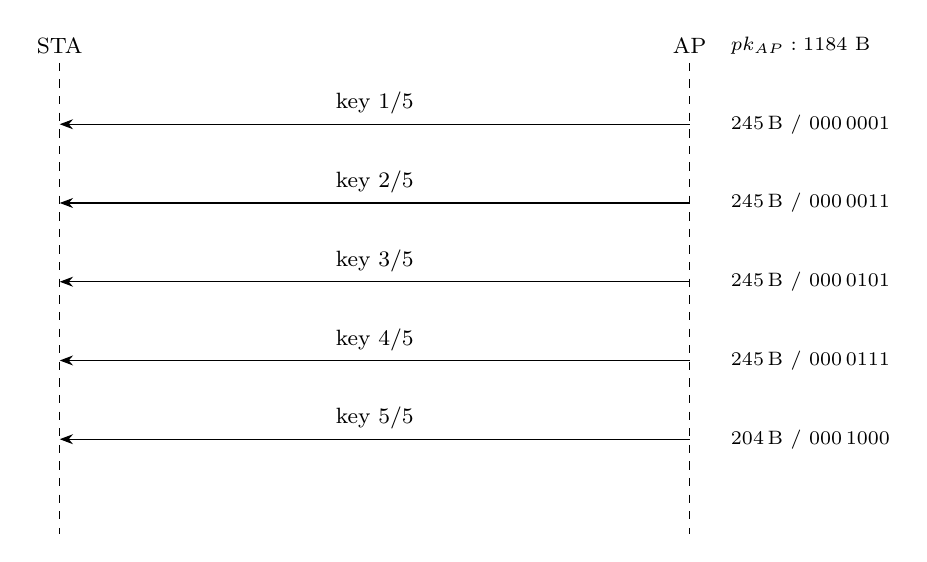
\begin{tikzpicture}[>=Stealth,font=\footnotesize]
\node (sta) at (0,0) {STA};
\node (ap)  at (8,0) {AP};
\draw[dashed] (sta)--(0,-6.2);
\draw[dashed] (ap)--(8,-6.2);
\node[right,font=\scriptsize] at (8.4,0) {$\pkAP:1184$ B};
\foreach \i/\y/\sz/\ctl in {1/-1/245/000\,0001,2/-2/245/000\,0011,3/-3/245/000\,0101,4/-4/245/000\,0111,5/-5/204/000\,1000}{
  \draw[->] (8,\y)--node[above]{key \i/5}(0,\y);
  \node[right,font=\scriptsize] at (8.4,\y) {\sz\,B / \ctl};
}
\end{tikzpicture}
\caption{Vendor Specific KDE 단편화 전송 (Control: Frag\#, More-bit)}\label{fig:frag}
\end{figure}

해당 프레임은 기존 WPA3와 동일하게 암호화되지 않은 상태로 전송되며, 무결성은
이후 Message~2의 MIC 검증과 키 파생 과정에서 간접적으로 보장된다. 또한
\pkAP{}/\ctSTA{}로 인해 프레임이 MTU를 초과하면 802.11 MAC 계층에서 자동
MPDU 단편화가 수행될 수 있으므로, 본 명세는 단편화 취약점 방어를 위해 파라미터
집합을 ML-KEM-768 이하로 제한한다(Section~\ref{sec:discussion}).

% =====================================================================
\section{EAPOL 4-Way Handshake 확장}\label{sec:eapol}
% =====================================================================
Figure~\ref{fig:msc}는 확장된 4-way handshake의 메시지 교환과 각 단계의 연산을
보인다.

\begin{figure}[H]\centering
\begin{tikzpicture}[>=Stealth,font=\footnotesize]
\node (sta) at (0,0.3) {\textbf{STA} (Supplicant)};
\node (ap)  at (10,0.3) {\textbf{AP} (Authenticator)};
\draw[dashed] (0,0)--(0,-8.4);
\draw[dashed] (10,0)--(10,-8.4);
\node[left,align=right,font=\scriptsize] at (9.8,-0.6)
  {$(\pkAP,\skAP)\leftarrow$ ML-KEM.KeyGen()};
\draw[->] (10,-1.1)--node[above]{\textbf{M1}: $\ANonce,\ \pkAP$}(0,-1.1);
\node[right,align=left,font=\scriptsize] at (0.2,-1.7)
  {$(\ctSTA,\ssK)\leftarrow$ ML-KEM.Encap($\pkAP$)};
\draw[->] (0,-2.6)--node[above]{\textbf{M2}: $\SNonce,\ \ctSTA,\ MIC_1$}(10,-2.6);
\node[left,align=right,font=\scriptsize] at (9.8,-3.2)
  {$\ssK\leftarrow$ ML-KEM.Decap($\skAP,\ctSTA$)};
\node[left,align=right,font=\scriptsize] at (9.8,-3.7)
  {$MIC_1$ 검증(SAE PMK), 이후 \ptkH{} 계산};
\draw[->] (10,-4.7)--node[above]{\textbf{M3}: $MIC_2,\ \{GTK\}$}(0,-4.7);
\node[right,align=left,font=\scriptsize] at (0.2,-5.3)
  {$MIC_2$ 검증 후 \ptkH{} 설치};
\draw[->] (0,-6.2)--node[above]{\textbf{M4}: $MIC_3$}(10,-6.2);
\draw[<->,thick] (0,-7.4)--node[above]{데이터 (GCMP-256, TK)}(10,-7.4);
\end{tikzpicture}
\caption{PQC 확장 EAPOL 4-way handshake 메시지 시퀀스}\label{fig:msc}
\end{figure}

\subsection{Message 1: AP $\to$ STA}
AP는 기존과 같이 \ANonce{}를 전송하는 동시에, 일회용 ML-KEM 키 쌍
$(\pkAP,\skAP)$를 생성하고 \pkAP{}를 EAPOL-Key의 Key Data 필드에
Vendor Specific KDE(PQC Subtype \hex{01})로 삽입한다. ML-KEM-768 기준 \pkAP{}의
크기는 1184 바이트이다. 이 프레임은 암호화되지 않은 상태로 전송된다.

\subsection{Message 2: STA $\to$ AP}
STA는 Message~1에서 \pkAP{}를 재조립한 뒤 ML-KEM 캡슐화를 수행하여 공유
비밀 \ssK{}과 암호문 \ctSTA{}를 생성한다(ML-KEM-768 기준 \ctSTA{}는 1088
바이트). 이후 STA는 \ssK{}과 \pmkSAE{}를 결합하여 \ptkH{}를 생성한다.

\begin{quote}\small
\textbf{MIC 검증 순서.} AP는 Message~2의 MIC를 확인하기 전까지 \ssK{}을 얻을
수 없으므로, Message~2의 1차 MIC($MIC_1$)는 SAE 기반 PMK에서 파생된 임시
KCK로 검증하고, decapsulation 이후 \ptkH{}로 전환한다. 이는 계산 비용이 큰
decapsulation을 MIC 검증 이전에 수행하지 않게 하여 DoS 공격을 방어한다
(Section~\ref{sec:dos}).
\end{quote}

Message~2에는 \ctSTA{} 뿐 아니라 Association 단계에서 협상된 RSN IE의 사본을
포함한다. 이를 통해 공격자가 Association 단계에서 PQC-AKM을 SAE-only 또는 낮은
보안 수준의 프로파일로 바꾸는 다운그레이드 공격을 탐지할 수 있다.

\subsection{Message 3 및 Message 4}
AP는 Message~2의 MIC를 검증한 뒤 \skAP{}로 \ctSTA{}를 decapsulation하여
\ssK{}을 획득하고, 동일한 $PRK$와 \ptkH{}를 계산한다. Message~3과
Message~4는 표준 WPA3 4-way handshake 절차를 따르되, MIC 및 후속 데이터
보호에는 \ptkH{}에서 파생된 $KCK,KEK,TK$를 사용한다. STA는 Message~3의 MIC
검증이 성공한 후 \ptkH{}를 최종적으로 설치한다.

% =====================================================================
\section{키 파생}\label{sec:kdf}
% =====================================================================
하이브리드 PTK는 HKDF~\cite{rfc5869}를 사용하여 다음과 같이 파생한다. HKDF-Extract
단계는 ML-KEM 공유 비밀과 SAE PMK을 IKM(Input Keying Material)으로 결합하고,
HKDF-Expand 단계가 최종 PTK를 생성한다.

\begin{align}
Salt &= \text{SHA-256}(\text{``WPA3-PQC-Hybrid''} \cat \ANonce \cat \SNonce) \label{eq:salt}\\
PRK  &= \text{HKDF-Extract}(Salt,\ IKM = \ssK \cat \pmkSAE) \label{eq:prk}\\
\ptkH &= \text{HKDF-Expand}(PRK,\ Info,\ L) \label{eq:ptk}
\end{align}
\begin{align}
Info =\ &\text{``Hybrid Pairwise key expansion''} \cat \min(AA,SPA) \cat \max(AA,SPA) \notag\\
        &\cat \min(\ANonce,\SNonce) \cat \max(\ANonce,\SNonce). \label{eq:info}
\end{align}

여기서 $AA$는 AP MAC 주소, $SPA$는 STA MAC 주소, $L$은 필요한 PTK 길이이다.
$Salt$에 \ANonce{}, \SNonce{}를 포함하는 이유는 세션마다 키 입력값을 달리하고
과거 키 재사용을 차단하기 위함이다. HKDF 해시는 프로파일에 따라 ML-KEM-512에서는
SHA-256, ML-KEM-768에서는 SHA-384를 사용한다. 단, $Salt$은 세션 구분과 nonce
바인딩을 위한 값이므로 SHA-256만으로도 충분하다.

식~(\ref{eq:ptk})에서 \ptkH{}를 계산하려면 $PRK$가 필요하고, $PRK$를 얻으려면
\pmkSAE{}와 \ssK{}을 모두 알아야 한다. 따라서 두 비밀 중 하나만 알고 있는
공격자는 유효한 PTK를 계산할 수 없다.

% =====================================================================
\section{보안 분석}\label{sec:security}
% =====================================================================
\subsection{수학적 근거: 하이브리드 결합기의 안전성}\label{sec:proof}
식~(\ref{eq:prk})의 결합 구조는 KEM 공유 비밀과 SAE PMK을 연결(concatenation)하여
HKDF-Extract에 입력하는 \emph{결합기(combiner)}이다. 본 절은 이 결합기가 두
입력 중 \emph{하나만} 안전해도 결과 키가 안전함을 보인다~\cite{giacon,bindel}.

\begin{assumption}[구성요소 안전성]\label{as:comp}
(i) ML-KEM은 IND-CCA2 안전한 KEM이며, 따라서 \ctSTA{}가 변조되지 않는 한 \ssK{}은
공격자에게 의사난수(pseudorandom)이다~\cite{fips203}. (ii) SAE는 오프라인 사전
공격에 저항적이며, 정당한 세션에서 \pmkSAE{}은 고전 공격자에게 의사난수이다~\cite{rfc7664}.
\end{assumption}

\begin{assumption}[HKDF 안전성]\label{as:hkdf}
HKDF-Extract의 기반 함수 HMAC은 dual-PRF(또는 랜덤 오라클)로 모델링된다.
즉 salt 또는 IKM 중 하나가 충분한 min-entropy를 가지면 출력 $PRK$는 균일
분포와 구분 불가류하다~\cite{rfc5869,sp80056c}.
\end{assumption}

\begin{theorem}[결합기 안전성]\label{thm:combiner}
가정~\ref{as:comp}과~\ref{as:hkdf} 하에서, \ssK{}과 \pmkSAE{} 중 적어도 하나가
공격자에게 계산적으로 알려지지 않으면, 식~(\ref{eq:prk})--(\ref{eq:ptk})로
파생된 \ptkH{}는 공격자에게 의사난수이다.
\end{theorem}

\begin{proof}[증명 개요]
IKM $=\ssK \cat \pmkSAE$ 에서 두 부분 중 하나가 의사난수이면 연결 문자열 전체도
충분한 min-entropy를 갖는다. 가정~\ref{as:hkdf}에 의해 HKDF-Extract 출력 $PRK$는
균일 분포와 구분 불가류하며, HKDF-Expand의 PRF 성질에 의해 \ptkH{} 역시
의사난수이다. 구체적으로, (a) 양자 공격자가 SAE(ECDH)를 깨더라도 ML-KEM의
IND-CCA2 안전성(가정~\ref{as:comp}(i))에 의해 \ssK{}이 보호되고, (b) ML-KEM
구현이 약화되더라도 SAE의 저항성(가정~\ref{as:comp}(ii))에 의해 \pmkSAE{}이
보호된다. 따라서 두 계열의 공격자 모두에 대해 적어도 하나의 비밀이 유지되므로
결과 키가 안전하다.
\end{proof}

\paragraph{암호문 바인딩.} 결합기가 ``하나만 안전해도 안전''한 강한 성질을
갖기 위해서는 KEM 암호문 \ctSTA{}이 파생 과정에 바인딩되어야 한다~\cite{giacon}.
본 설계에서 \ctSTA{}은 Message~2의 MIC로 무결성이 보호되므로, 공격자가 암호문을
변조하거나 재사용하면 MIC 검증이 실패한다. 방어 심화를 위해 향후 개정에서는
$H(\ctSTA)$를 $Info$에 추가하는 것을 고려할 수 있다.

\subsection{위협 모델 및 대응}
Table~\ref{tab:threat}은 제안 방식이 고려하는 주요 공격 벡터와 방어 기제를
정리한다.

\begin{table}[H]\centering
\caption{보안 위협 및 방어 기제}\label{tab:threat}
\small
\renewcommand{\arraystretch}{1.15}
\begin{tabularx}{\linewidth}{@{}p{20mm}XX@{}}
\toprule
공격 벡터 & 공격 시나리오 & 방어 기제 \\ \midrule
패킷 위변조 & 캡처한 공개키/암호문을 변조하여 주입
  & SAE 기반 PMK 또는 hybrid PTK로 MIC를 검증하므로 변조된 프레임은 상태
    머신에서 폐기 \\
패킷 재전송 & 과거 EAPOL 프레임을 현재 세션에 재주입
  & Replay Counter 검증 및 $Salt$에 \ANonce/\SNonce{}를 결합하여 과거 키
    재사용 차단 \\
다중 채널 조작 & 다른 채널의 가짜 AP 릴레이 공격
  & Operating Channel Validation(OCV)으로 채널 정보를 MIC 계산에 포함 \\
저장 후 해독 & 현재 트래픽 저장 후 미래 양자 컴퓨터로 SAE PMK 해독
  & 일회용 ML-KEM 공유 비밀과 PMK을 결합하여 데이터 키 파생 (Section~\ref{sec:fs}) \\
중간자 공격 & \pkAP{}/\ctSTA{}를 각각 위조하여 양측과 별도 비밀 형성
  & EAPOL MIC가 PMK 및 hybrid PTK에 바인딩 (Section~\ref{sec:mitm}) \\
\bottomrule
\end{tabularx}
\end{table}

\subsection{MIC 검증 순서와 DoS 방어}\label{sec:dos}
EAPOL 처리에서는 계산 비용이 큰 decapsulation을 수행하기 전에 MIC를 검증하는 것이
중요하다. 만약 AP가 MIC 검증 전에 임의의 \ctSTA{}를 decapsulation한다면,
공격자는 대량의 위조 암호문을 전송하여 AP의 계산 자원을 고갈시키는 DoS
공격을 수행할 수 있다. 따라서 본 설계에서는 Message~2의 처리 순서를 MIC 검증
이후 decapsulation으로 제한한다. 이때 AP는 아직 \ssK{}을 알 수 없으므로,
Message~2의 1차 MIC 검증은 SAE 기반 PMK에서 파생된 임시 KCK로 수행하고,
decapsulation 이후 hybrid PTK를 계산한다.

\subsection{중간자 공격 저항성}\label{sec:mitm}
공격자 Mallory가 AP와 STA 사이에서 AP의 \pkAP{}를 자신의 $pk'$로 교체한다고
가정한다. STA는 $pk'$에 대해 캡슐화를 수행하여 $ss'$와 $ct'$를 생성할 수
있다. 그러나 Mallory가 AP를 속이려면 Message~2 내부의 \ctSTA{}를 AP의 실제
\pkAP{}에 대응하는 암호문으로 교체해야 한다. 이 경우 프레임 내용이 변경되므로
새로운 MIC가 필요하지만, Mallory는 \pmkSAE{}를 알지 못해 유효한 MIC를 생성할 수
없다. 따라서 AP는 변조된 Message~2를 decapsulation 이전에 폐기한다.

만약 Mallory가 $ct'$를 그대로 AP에 전달하더라도 AP의 \skAP{}로는 올바른
$ss$를 복구할 수 없다. 이 경우 AP와 STA가 서로 다른 공유 비밀을 사용하여
Message~3의 MIC를 계산하게 되므로, STA MIC 검증 단계에서 handshake가
중단된다.

\subsection{순방향 비밀성}\label{sec:fs}
본 설계는 세션마다 일회용 ML-KEM 키 쌍 $(\pkAP,\skAP)$를 생성한다. 따라서
특정 세션의 임시 ML-KEM 개인키가 삭제된 이후에는, 장기 PMK이 노출되더라도
과거 세션의 \ssK{}을 복원하기 어렵다. 결과적으로 hybrid PTK는 SAE 기반
보안성과 PQC 기반 임시 공유 비밀에 동시에 의존하며, 저장 후 해독 공격에 대한
저항성을 제공한다.

% =====================================================================
\section{구현 및 실험 평가}\label{sec:impl}
% =====================================================================

\subsection{구현 환경 및 라이브러리 버전}
Table~\ref{tab:env}에 검증에 사용한 구성요소와 버전을 기록한다(재현성을 위해
커밋 해시까지 명시).

\begin{table}[H]\centering
\caption{구현 및 검증 환경 (값을 채워 넣을 것)}\label{tab:env}
\small
\begin{tabularx}{\linewidth}{@{}lX@{}}
\toprule
구성요소 & 버전 / 커밋 \\ \midrule
hostapd / wpa\_supplicant (hostap-pqc) & \textit{ca266cc24d8705eb1a2a0857ad326e48b1408b20} \\
ML-KEM 구현 (liboqs-80211) & \textit{liboqs 0.15.0} \\
펌웨어 / OS (openwrt-pqc) & \textit{openwrt 25.12} \\
하드웨어 플랫폼 (AP/STA) & \textit{ipTIME AX3000SE, SoC : MT7981BA ,RAM : DDR3 256MB, NAND : 128MB} \\
\bottomrule
\end{tabularx}
\end{table}

\subsection{기능 검증}
확장된 4-way handshake가 정상적으로 완료되고 hybrid PTK가 설치되는지,
그리고 이후 데이터 프레임이 GCMP-256으로 정상 복호화되는지를 검증한다. 변경
사항은 \code{main}(원본) 대비 \code{master}(최종 산출물)의 git diff
(\code{diff\_output.txt})로 첨부한다.

\begin{table}[H]\centering
\caption{기능 검증 항목}\label{tab:func}
\small
\begin{tabularx}{\linewidth}{@{}Xcc@{}}
\toprule
항목 & 기대 결과 & 실측 \\ \midrule
Association PQC-AKM 협상 & \code{00-0F-AC:32} 선택 & \textit{성공} \\
M1 \pkAP{} 단편 수신/재조립 & 5 조각 재조립 성공 & \textit{성공} \\
M2 \ctSTA{} 단편 전송 & 5 조각 전송 성공 & \textit{성공} \\
Hybrid PTK 설치 & M1--M4 완료 & \textit{성공} \\
데이터 프레임 복호화(Wireshark) & 복호화 성공 & \textit{성공} \\
\bottomrule
\end{tabularx}
\end{table}

\subsection{성능 평가}
Table~\ref{tab:perf}는 기존 WPA3-SAE 대비 추가 오버헤드 측정 항목이다(평균 및
표준편차, 최소 100회 반복 권장). - 본 문서에서는 측정값을 생략한다.

\begin{table}[H]\centering
\caption{성능 오버헤드 (측정값을 채워 넣을 것)}\label{tab:perf}
\small
\begin{tabular}{@{}lcc@{}}
\toprule
지표 & WPA3-SAE(기준) & WPA3-PQC(제안) \\ \midrule
Handshake 지연(ms) & \textit{생략} & \textit{생략} \\
EAPOL M1 크기(B) & \textit{생략} & \textit{생략} \\
EAPOL M2 크기(B) & \textit{생략} & \textit{생략} \\
총 추가 전송량(B) & N/A & \textit{생략} \\
KDE 조각 수(M1/M2) & N/A & 5 / 5 \\
CPU(KeyGen/Encap/Decap, ms) & N/A & \textit{생략} \\
\bottomrule
\end{tabular}
\end{table}

% =====================================================================
\section{논의}\label{sec:discussion}
% =====================================================================
제안 방식은 새로운 IE를 정의하지 않고 RSN IE의 AKM Suite 확장만으로 PQC 지원
여부를 협상한다는 점에서 기존 IEEE 802.11 관리 프레임 구조와의 호환성이 높다.
또한 ML-KEM 공개키와 암호문을 Vendor Specific KDE로 분할 전송하므로 EAPOL-Key
프레임의 Key Data 구조를 크게 변경하지 않는다. 다만 ML-KEM-768 공개키(1184 B)와
암호문(1088 B)은 각각 1 KB 이상이므로, 구현 시 프레임 크기, 조각 순서 검증,
재조립 버퍼 관리, replay counter 연동, 그리고 단편화 취약점 방어를 함께
고려해야 한다.

MTU 초과를 방지하기 위해 본 설계는 ML-KEM-768을 상한 프로파일로 설정한다. 더 큰
PQC KEM(예: ML-KEM-1024)을 사용하는 경우 802.11 MAC 단편화가 발생할 수 있으며,
이는 구현 복잡성과 공격 표면을 증가시킬 수 있다. 따라서 실제 표준화 또는 구현
단계에서는 조각 수 제한, 최대 Key Data 길이, 잘못된 fragment 순서에 대한 즉시 폐기
정책을 명확히 정의해야 한다.

% =====================================================================
\section{결론}
% =====================================================================
본 명세는 WPA3-SAE의 Authentication 절차를 유지하면서 Association 및 EAPOL 4-way
handshake에 PQC(ML-KEM) 하이브리드 키 교환을 통합하는 구조를 정의하였다. RSN
IE의 AKM Suite 확장을 통해 ML-KEM-768 및 ML-KEM-512 프로파일을 협상하고, EAPOL
Message~1과 Message~2에서 ML-KEM 공개키와 암호문을 교환한 뒤 \pmkSAE{}와
\ssK{}을 HKDF로 결합하여 hybrid PTK를 생성한다. 제안 방식은 기존 WPA3 상태
머신의 MIC 검증 원칙을 보존하면서, 저장 후 해독 공격과 양자 컴퓨팅 기반 장기
위험에 대한 방어력을 강화한다. 향후 작업으로는 Section~\ref{sec:impl}의 실측
결과 보강과 암호문 바인딩 강화($H(\ctSTA)$ 포함)가 있다.

% =====================================================================
\begin{thebibliography}{99}
\bibitem{ieee80211} IEEE, ``IEEE Std 802.11-2020: Wireless LAN Medium Access
  Control (MAC) and Physical Layer (PHY) Specifications,'' 2021.
  (9.4.2.24.3 AKM suites, Table 9-151; Clause 12 RSNA / EAPOL-Key, KDE)
\bibitem{fips203} NIST, ``FIPS 203: Module-Lattice-Based Key-Encapsulation
  Mechanism Standard,'' Aug. 2024.
\bibitem{rfc5869} H. Krawczyk and P. Eronen, ``HMAC-based Extract-and-Expand
  Key Derivation Function (HKDF),'' RFC 5869, May 2010.
\bibitem{rfc7664} D. Harkins, ``Dragonfly Key Exchange,'' RFC 7664, Aug. 2015.
\bibitem{ieee8021x} IEEE, ``IEEE Std 802.1X-2020: Port-Based Network Access
  Control,'' 2020.
\bibitem{sp80056c} NIST, ``SP 800-56C Rev. 2: Recommendation for Key-Derivation
  Methods in Key-Establishment Schemes,'' Aug. 2020.
\bibitem{wpa3} Wi-Fi Alliance, ``WPA3 Specification,'' Version 3.x.
\bibitem{giacon} F. Giacon, F. Heuer, and B. Poettering, ``KEM Combiners,''
  PKC 2018, LNCS 10769, pp. 190--218.
\bibitem{bindel} N. Bindel, J. Brendel, M. Fischlin, B. Goncalves, and
  D. Stebila, ``Hybrid Key Encapsulation Mechanisms and Authenticated Key
  Exchange,'' PQCrypto 2019, LNCS 11505, pp. 206--226.
\end{thebibliography}

\end{document}